\section{Constitutional AI and Scalable Oversight}

\begin{frame}{}
    \LARGE Alignment and Post-Training: \textbf{Constitutional AI and Scalable Oversight}

    \vspace{1em}
    \normalsize How do you supervise a model that knows more than its supervisor?
\end{frame}

\begin{frame}{Constitutional AI in One Slide (Recap)}
    \centering
    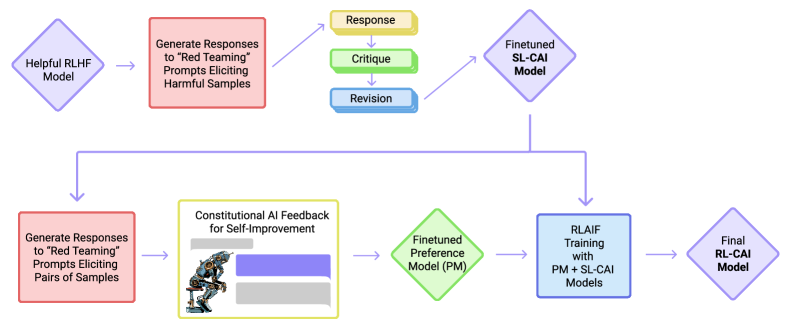
\includegraphics[width=0.8\linewidth,height=0.39\textheight,keepaspectratio]{images/alignment-post-training/cai_fig1_two_stages.png}
    \begin{itemize}\itemsep0.3em
        \item \textbf{The idea.} Replace harmlessness labels with a written list of principles, and have the model apply them to itself.
        \item \textbf{Stage 1.} Self-critique and revision against a sampled principle, then SFT on the revisions.
        \item \textbf{Stage 2.} AI-labelled preferences train a preference model, then RL against it.
    \end{itemize}
    \vspace{0.1em}
    \takeaway{In 2022 the constitution was used only to \emph{make labels}. Where did it go next?}
    \src{Bai et al., ``Constitutional AI: Harmlessness from AI Feedback,'' \href{https://arxiv.org/abs/2212.08073}{arXiv:2212.08073}, Figure 1. Recap of the KAUST Academy LLM course.}
\end{frame}

\begin{frame}{Beyond CAI: Teach the Model to Reason with the Specification}
    \begin{columns}[T,onlytextwidth]
        \column{0.58\textwidth}
        \textbf{Deliberative alignment} (OpenAI, o1 and o3-mini)
        \begin{enumerate}\itemsep0.3em
            \item Pair each prompt with the section of the safety specification for its category.
            \item A reasoning model writes a chain of thought that \emph{cites the policy}.
            \item A judge that sees the specification filters the results.
            \item \textbf{Strip the specification} from the prompt, then run SFT on prompt, reasoning and answer.
            \item RL, with the specification-aware judge as reward. The reasoning is hidden from the judge.
        \end{enumerate}
        \column{0.4\textwidth}
        \centering
        \small
        \begin{adjustbox}{max width=\linewidth}\begin{tabular}{lcc}
            \toprule
            & \textbf{o1} & \textbf{GPT-4o} \\
            \midrule
            StrongREJECT & 0.88 & 0.37 \\
            \bottomrule
        \end{tabular}\end{adjustbox}

        \vspace{0.3em}
        {\scriptsize Jailbreak robustness (goodness@0.1). o1 also scores 0.93 on XSTest, which measures over-refusal.}

        \vspace{0.8em}
        \begin{itemize}\itemsep0.3em
            \item No human-labelled completions are needed.
            \item Both the SFT and the RL stage contribute.
        \end{itemize}
    \end{columns}
    \vspace{0.3em}
    \takeaway{CAI uses the specification to produce labels. Deliberative alignment puts the specification's text \textbf{into the policy's own reasoning}.}
    \src{Guan et al., ``Deliberative Alignment: Reasoning Enables Safer Language Models,'' \href{https://arxiv.org/abs/2412.16339}{arXiv:2412.16339}, Figures 2 and 14.}
\end{frame}

\begin{frame}{Constitutions as Safeguards and as Public Documents}
    \begin{center}
    \small
    \begin{adjustbox}{max width=\linewidth}\begin{tabular}{lcc}
        \toprule
        \textbf{Constitutional Classifiers} & \textbf{2025} & \textbf{2026 (++)} \\
        \midrule
        Inference overhead & 23.7\% & about 1\% \\
        Extra refusals on production traffic & 0.38\% & 0.05\% \\
        Universal jailbreak found by red-teamers & none & none \\
        \bottomrule
    \end{tabular}\end{adjustbox}
    \end{center}
    \begin{itemize}\itemsep0.35em
        \item A constitution of allowed and disallowed content drives \textbf{synthetic data} to train input and streaming output classifiers. Automated jailbreak success fell from 86\% to about 4.4\%.
        \item The 2026 version adds a two-stage cascade and \textbf{linear probes on activations}. Cheap enough to run on all traffic.
    \end{itemize}
    \begin{center}
    \small
    \begin{adjustbox}{max width=\linewidth}\begin{tabular}{>{\raggedright\arraybackslash}p{3.6cm}>{\raggedright\arraybackslash}p{9.7cm}}
        \toprule
        Claude's constitution (Jan 2026) & priority order: broadly safe, broadly ethical, follows guidelines, helpful. Plus hard constraints. Claude generates synthetic training data from it \\
        OpenAI Model Spec (Aug 2026) & chain of command: root, system, developer, user, guideline. Tool outputs are untrusted by default \\
        \bottomrule
    \end{tabular}\end{adjustbox}
    \end{center}
    \src{Anthropic, ``Constitutional Classifiers,'' \href{https://arxiv.org/abs/2501.18837}{arXiv:2501.18837}. Cunningham et al., ``Constitutional Classifiers++,'' \href{https://arxiv.org/abs/2601.04603}{arXiv:2601.04603}. Anthropic, ``Claude's new constitution'' (2026). OpenAI Model Spec (2026-08-18).}
\end{frame}

\begin{frame}{Why Oversight Must Scale: Sandwiching}
    \begin{columns}[T,onlytextwidth]
        \column{0.5\textwidth}
        \begin{itemize}\itemsep0.5em
            \item A specification needs someone to check that the model follows it. What if the checker is the weakest party?
            \item \textbf{Sandwiching} sets up the experiment today:
            \begin{itemize}\itemsep0.25em
                \item \textbf{Non-experts:} aligned, but lack the skill.
                \item \textbf{Model:} has the skill, not reliably aligned.
                \item \textbf{Experts:} used only to score the outcome.
            \end{itemize}
            \item Can the non-expert, using the model, beat both the model and themselves?
        \end{itemize}
        \column{0.48\textwidth}
        \centering
        \small
        \begin{adjustbox}{max width=\linewidth}\begin{tabular}{lcc}
            \toprule
            \textbf{Accuracy (\%)} & \textbf{MMLU} & \textbf{QuALITY} \\
            \midrule
            Human alone & 57.2 & 48.6 \\
            Model alone & 65.6 & 66.9 \\
            \rowcolor{KAUSTcyan!12} Human with model & 75.4 & 76.8 \\
            Expert estimate & 90.0 & 93.5 \\
            \bottomrule
        \end{tabular}\end{adjustbox}

        \vspace{0.6em}
        {\scriptsize Model: best-of-20 with chain of thought. QuALITY is time-limited.}
    \end{columns}
    \vspace{0.4em}
    \takeaway{The team beats both parts, but stays far from the expert. The authors call the result too weak for high-stakes use.}
    \src{Bowman et al., ``Measuring Progress on Scalable Oversight for Large Language Models,'' \href{https://arxiv.org/abs/2211.03540}{arXiv:2211.03540}, Table 1.}
\end{frame}

\begin{frame}{Debate: Let Two Models Argue, and Judge the Argument}
    \begin{columns}[T,onlytextwidth]
        \column{0.56\textwidth}
        \begin{itemize}\itemsep0.4em
            \item \textbf{Theory (2018).} With optimal play, a polynomial-time judge of a debate decides PSPACE questions. Direct judging corresponds to NP.
            \item \textbf{Evidence (2024).} Debaters read a story. The judge sees only arguments and verified quotes.
            \item More persuasive debaters make judges \textbf{more} accurate.
            \item A more persuasive single consultant makes judges \alert{less} accurate.
        \end{itemize}
        \column{0.42\textwidth}
        \centering
        \small
        \begin{adjustbox}{max width=\linewidth}\begin{tabular}{lcc}
            \toprule
            \textbf{Judge accuracy} & \textbf{LLM} & \textbf{Human} \\
            \midrule
            No help & 48\% & 60\% \\
            Consultancy & n/a & 78\% \\
            \rowcolor{KAUSTcyan!12} Debate & 76\% & 88\% \\
            \bottomrule
        \end{tabular}\end{adjustbox}
    \end{columns}
    \vspace{0.5em}
    \begin{itemize}\itemsep0.4em
        \item \textbf{The limits.} Across more tasks, debate beat direct answering only where debaters hold information the judge lacks. In a 2026 study, a single independent critique recovered most of its benefit.
    \end{itemize}
    \src{Irving, Christiano, Amodei, ``AI safety via debate,'' \href{https://arxiv.org/abs/1805.00899}{arXiv:1805.00899}. Khan et al., ``Debating with More Persuasive LLMs Leads to More Truthful Answers,'' \href{https://arxiv.org/abs/2402.06782}{arXiv:2402.06782}. Kenton et al., \href{https://arxiv.org/abs/2407.04622}{arXiv:2407.04622}. Elasky et al., \href{https://arxiv.org/abs/2605.27483}{arXiv:2605.27483}.}
\end{frame}

\begin{frame}{Weak-to-Strong Generalisation}
    \begin{columns}[T,onlytextwidth]
        \column{0.45\textwidth}
        \centering
        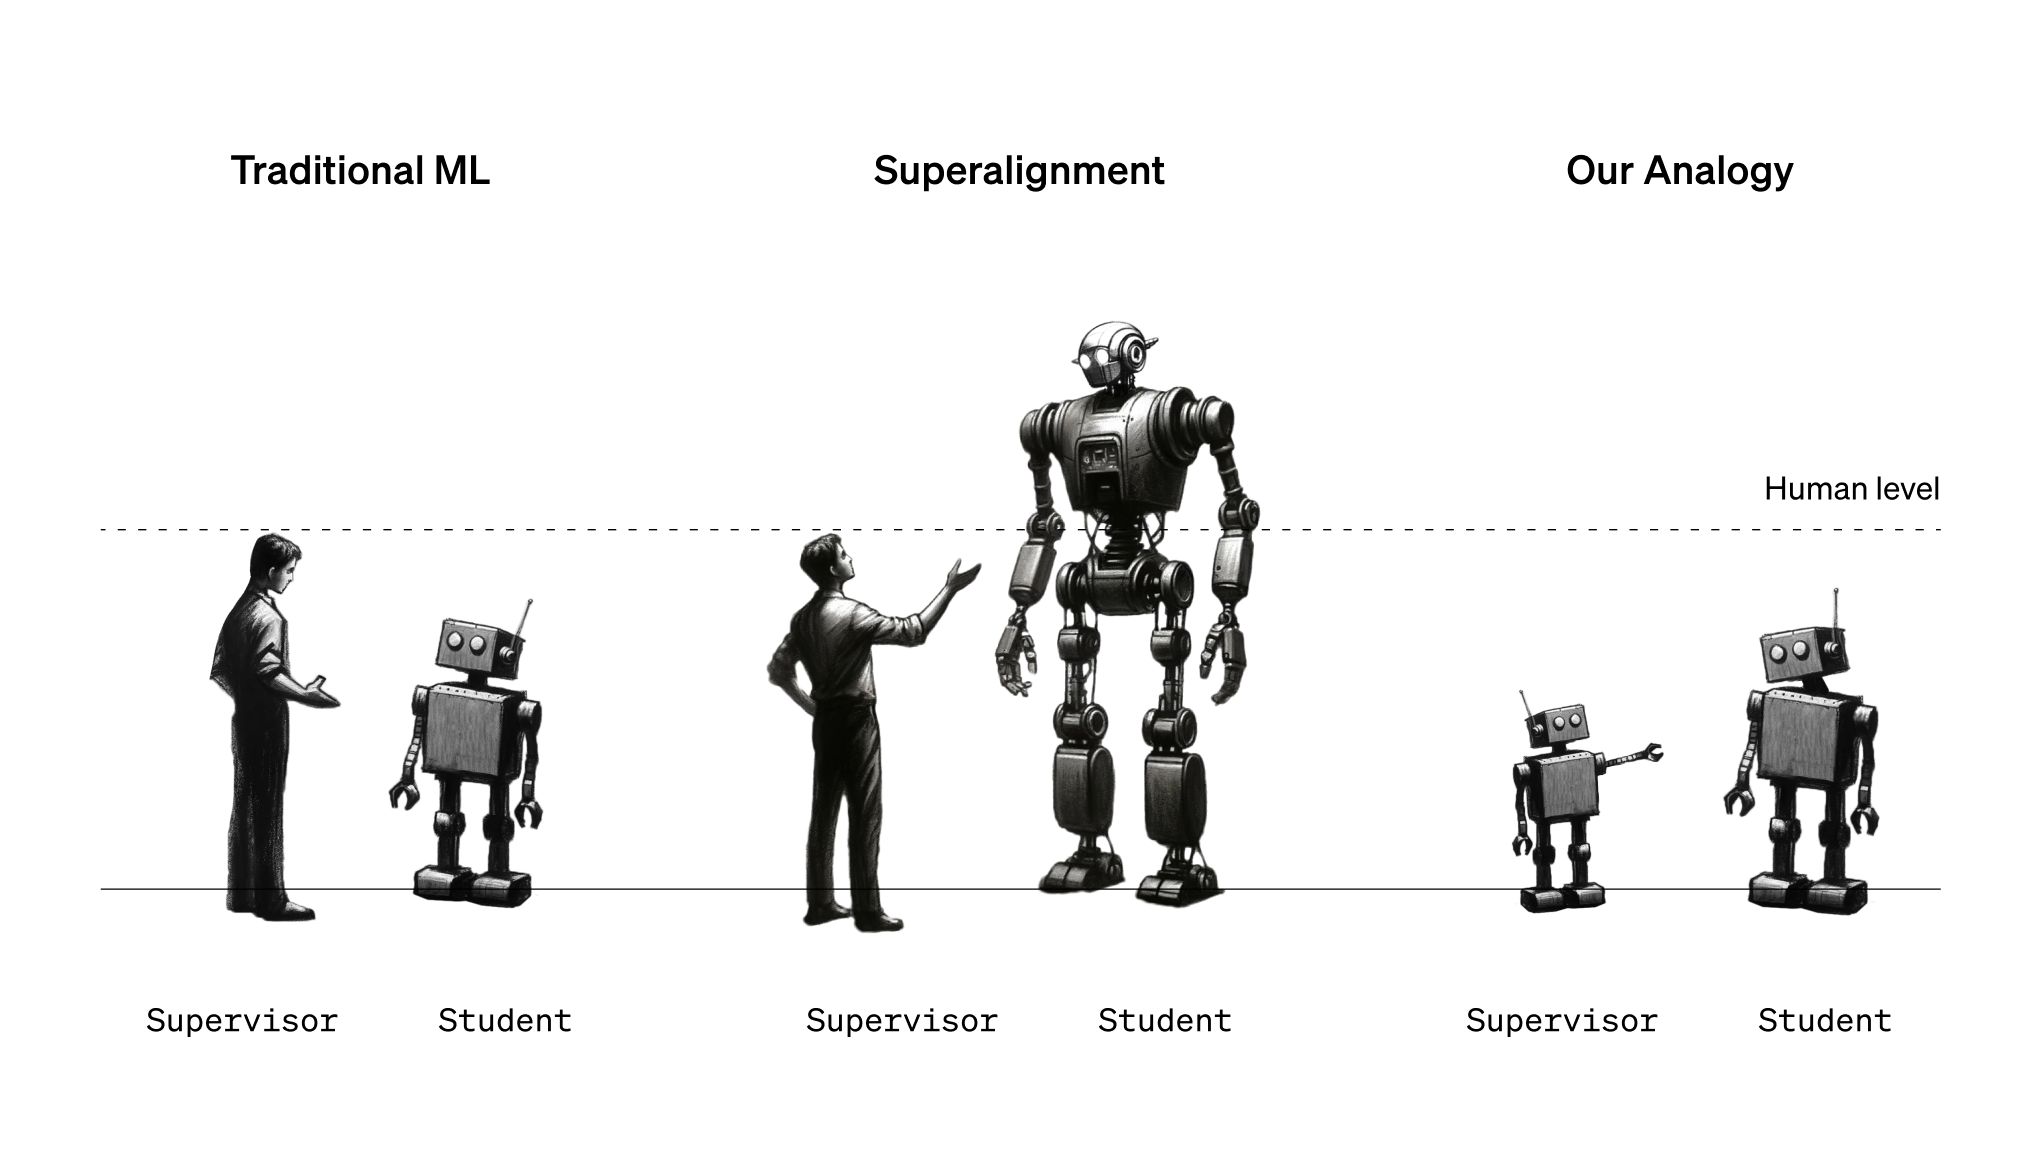
\includegraphics[width=\linewidth,height=0.34\textheight,keepaspectratio]{images/alignment-post-training/w2s_fig1_analogy.png}
        {\footnotesize\[
            \text{PGR}=\frac{\text{weak-to-strong}-\text{weak}}{\text{strong ceiling}-\text{weak}}
        \]}
        \column{0.53\textwidth}
        \begin{itemize}\itemsep0.4em
            \item \textbf{Setup.} Fine-tune a strong model on a weak supervisor's labels. Does it copy the errors, or generalise past them?
            \item \textbf{PGR:} 0 if the student only matches its teacher, 1 if it reaches its own ceiling.
            \item \textbf{A confidence loss} adds the student's own hardened predictions:
            {\footnotesize\[
                \mathcal{L}=(1-\alpha)\,\mathrm{CE}\big(f(x),f_w(x)\big)+\alpha\,\mathrm{CE}\big(f(x),\hat f_t(x)\big)
            \]}
            \item With the smallest supervisor and largest student, median PGR on 22 NLP tasks rises from about 25\% to nearly 80\%.
        \end{itemize}
    \end{columns}
    \vspace{0.2em}
    \caveat{For \textbf{reward modelling}, naive PGR is usually about 10\% and almost never exceeds 20\%.}
    \src{Burns et al., ``Weak-to-Strong Generalization: Eliciting Strong Capabilities With Weak Supervision,'' \href{https://arxiv.org/abs/2312.09390}{arXiv:2312.09390}, Figure 1 and Appendix A.4.}
\end{frame}

\begin{frame}{Critics: Train a Model to Find the Flaws}
    \begin{columns}[T,onlytextwidth]
        \column{0.42\textwidth}
        \centering
        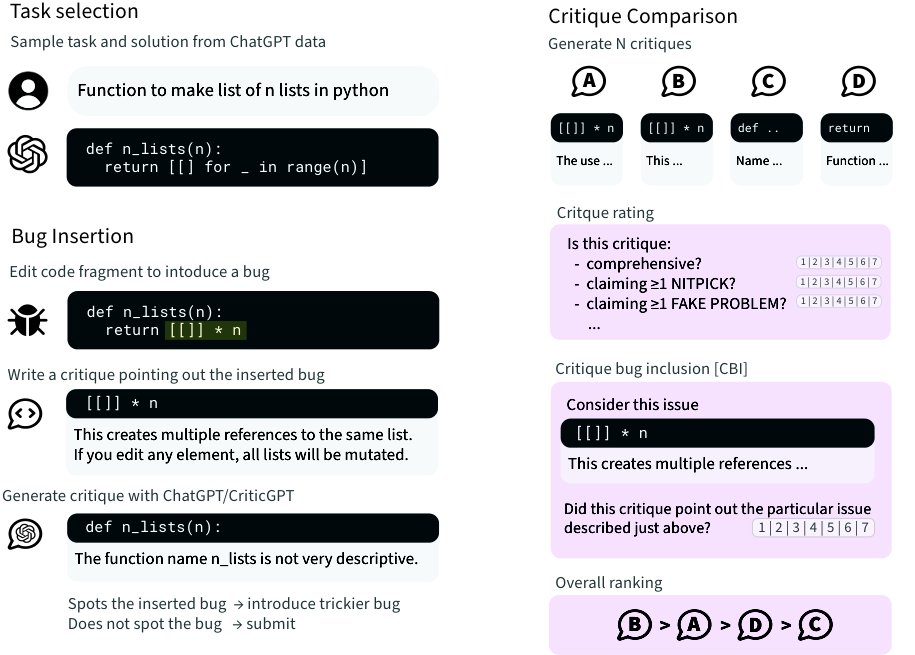
\includegraphics[width=\linewidth,height=0.62\textheight,keepaspectratio]{images/alignment-post-training/criticgpt_fig3_tampering_pipeline.png}
        \column{0.56\textwidth}
        \begin{itemize}\itemsep0.45em
            \item \textbf{Goal.} A critic model that reviews model-written code, so that human raters catch more bugs.
            \item \textbf{Tampering data.} Contractors insert subtle bugs and write the matching review. A bug is kept only if it evades an existing critic at least 33\% of the time.
            \item \textbf{CriticGPT} is trained with RLHF on these.
            \item Its critiques are preferred over human critiques \alert{63\%} of the time on naturally occurring bugs.
            \item Critics found problems in \alert{24\%} of training data that humans had rated flawless.
            \item Humans working \emph{with} the critic move beyond the frontier of the model alone. Hallucinated bugs and nitpicks remain ``quite high''.
        \end{itemize}
    \end{columns}
    \vspace{0.2em}
    \src{McAleese et al., ``LLM Critics Help Catch LLM Bugs,'' \href{https://arxiv.org/abs/2407.00215}{arXiv:2407.00215}, Figure 3.}
\end{frame}

\begin{frame}{Legibility: An Answer the Supervisor Can Check}
    \begin{itemize}\itemsep0.4em
        \item \textbf{The legibility tax.} Optimise a model for correctness alone and its solutions become hard to check. Time-limited humans lost \alert{32 to 50\%} accuracy when judging solutions from late in training.
        \item \textbf{Prover-verifier games.} A \emph{helpful} prover and a \emph{sneaky} prover write solutions for a much smaller verifier, about $10^{-3}$ of their compute. The reward is the verifier's score, signed by role and correctness:
    \end{itemize}
    \[
        R(z\mid x,\text{role})=
        \begin{cases}
            \big(2\cdot\mathbb{1}_{\text{correct}}(x,z)-1\big)\big(2\cdot\mathbb{1}_{\text{helpful}}(\text{role})-1\big)\,V'(x,z), & V'>0\\
            -1, & \text{otherwise}
        \end{cases}
    \]
    \begin{itemize}\itemsep0.4em
        \item After five rounds, human accuracy on the helpful prover's solutions recovers. The sneaky prover's errors become subtler round by round.
    \end{itemize}
    \vspace{0.2em}
    \takeaway{As with debate and tampering: \textbf{adversarial} signals hold up where cooperative ones erode.}
    \src{Kirchner et al., ``Prover-Verifier Games Improve Legibility of LLM Outputs,'' \href{https://arxiv.org/abs/2407.13692}{arXiv:2407.13692}, Figure 8.}
\end{frame}

\begin{frame}{Oversight: What to Remember}
    \begin{center}
    \small
    \begin{adjustbox}{max width=\linewidth}\begin{tabular}{lll}
        \toprule
        \textbf{Protocol} & \textbf{Works when} & \textbf{Known limit} \\
        \midrule
        Specification in training & the policy can reason with the text & models ``do not yet fully reflect'' it \\
        Debate & debaters hold evidence the judge lacks & one critique gives most of the benefit \\
        Weak-to-strong & classification, with a confidence loss & reward modelling recovers little \\
        Critics & bugs can be inserted to make data & nitpicks and hallucinated bugs \\
        Prover-verifier & an adversary is trained alongside & a legibility tax \\
        \bottomrule
    \end{tabular}\end{adjustbox}
    \end{center}
    \begin{itemize}\itemsep0.4em
        \item The shared assumption, stated openly in recursive reward modelling: \textbf{evaluation is easier than generation}.
    \end{itemize}
    \takeaway{\textbf{Next.} Constitutions, critics and classifiers all ran on \emph{synthetic data}. Time to look at how that data is made.}
    \src{Leike et al., ``Scalable agent alignment via reward modeling,'' \href{https://arxiv.org/abs/1811.07871}{arXiv:1811.07871}. OpenAI Model Spec (2026-08-18).}
\end{frame}
